% This text is proprietary.
% It's a part of presentation made by myself.
% It may not used commercial.
% The noncommercial use such as private and study is free
% Sep. 2005
% Author: Sascha Frank
% University Freiburg
% www.informatik.uni-freiburg.de/~frank/


\documentclass{beamer}
\usepackage{graphicx}

%%%%%%%%%%%%%%%%%%%%%%%%%%%%MACROS

\def\var#1{\mbox{\textrm{\bf{\sc{#1}}}}}
\newcommand{\set}[1]{\{#1\}}
\newcommand{\V}{\mathbb{V}}
\newcommand{\E}{\mathbb{E}}
\newcommand{\size}[1]{\ensuremath{\left|#1\right|}}

\newcommand {\framedgraphic}[3] {
    \frame{\frametitle{#1}
        \begin{center}
            \includegraphics[width=\textwidth,height=#3\textheight,keepaspectratio]{#2}
        \end{center}
    }
}
\newcommand{\disableframe}[1]{}

\def\func#1#2{\mbox{\textrm{\bf{\sc{#1}}}}\ensuremath{(~{#2}~)}}
% pseudocode notations
\newcommand{\T}{\mbox{\hspace{0.5cm}}}

% asymptotic notations
\newcommand{\Oh}[1]{\ensuremath{{\mathcal O}\left({#1}\right)}}
\newcommand{\Om}[1]{\ensuremath{{\Omega}\left({#1}\right)}}
\newcommand{\Th}[1]{\ensuremath{{\Theta}\left({#1}\right)}}

\newcommand{\ceil}[1]{\ensuremath{\left\lceil#1\right\rceil}}
\newcommand{\floor}[1]{\ensuremath{\left\lfloor#1\right\rfloor}}
\newcommand{\maybepause}{
    \iffalse
    \pause
    \fi
}

%%%%%%%%%%%%%%%%%%%%%%%%%%%%MACROS

\begin{document}
\title{A new optimal algorithm for parallel level synchronous BFS in the Cilk model}
\author{Yonatan R. Fogel}
\date{\today}

\frame{\titlepage}

%TODO: Maybe re-add table of contents
%\frame{\frametitle{Table of contents}\tableofcontents}

\section{Introduction}
\frame{\frametitle{BFS}
    \begin{itemize}
        \item Given
            \begin{itemize}
                \item Graph $G=(\V,\E)$ with diameter $D$
                \item Source vertex $s \in \V$
            \end{itemize}
        \item Calculate
            \begin{itemize}
                \item $Dist_{u\in \V} =$ length of the shortest path from $s$ to $u$ in $G$
%                \item $Parent_{u\in \V} = v \in \V$ s.t. $(v, u) \in \E, Dist_u = Dist_v + 1$
            \end{itemize}

        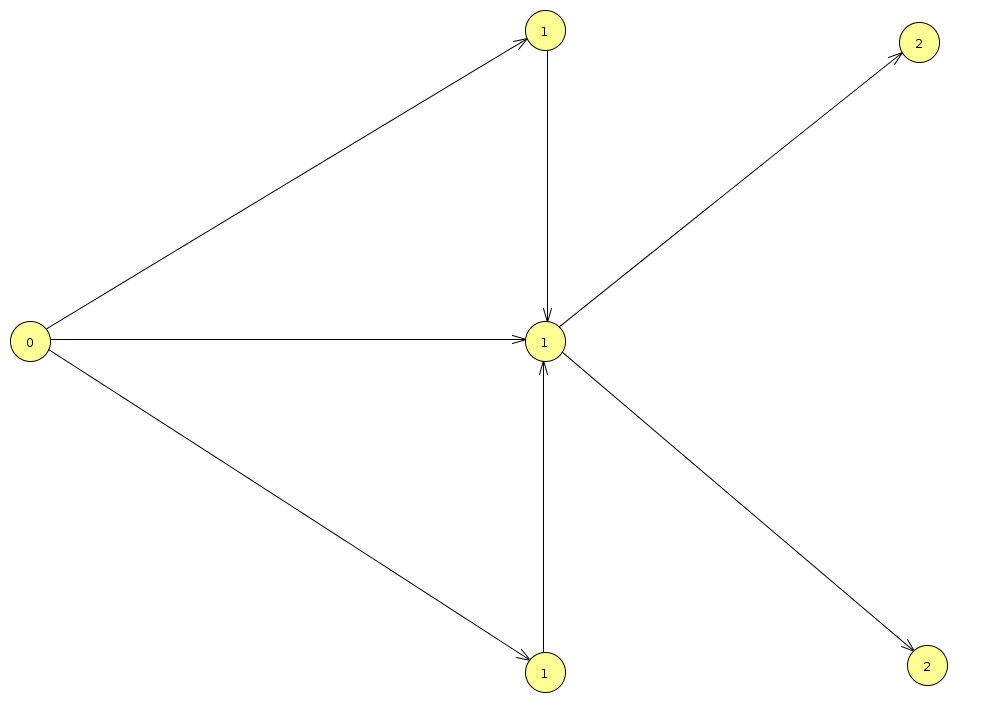
\includegraphics[width=\textwidth,height=0.5\textheight,keepaspectratio]{bfs-1.png}
    \end{itemize}
}

\frame{\frametitle{Parallel BFS}
    \begin{itemize}
        \item The runtime for serial BFS is $T_s=\Th{\size{\V}+\size{\E}}$
        \item For large graphs, calculating $Dist$ can be slow
        \item We can speed up BFS by processing edges and/or nodes in parallel
        \item Our new TBN-BFS achieves near-perfect linear speadup when $p \ll \frac{\size{V}+\size{E}}{D\log\left(\size{V}+\size{E}\right)}$

            \bigskip
            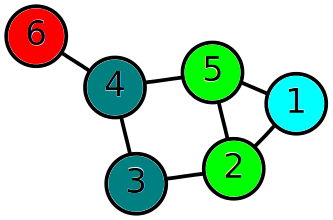
\includegraphics[width=\textwidth,height=0.25\textheight,keepaspectratio]{6n-graf.png}
    \end{itemize}
}

\frame{\frametitle{Level-Synchronous BFS}
    \begin{itemize}
        \item All nodes at distance $d$ from $s$ are processed before any nodes at distance $d^\prime > d$ \maybepause
        \item Level-Synchronous BFS has lower bounds of
            \begin{itemize}
                \item $T_p = \Om{\frac{\size{\V}+\size{\E}}{p}+D}$
                \item $T_1,W_p = \Om{T_s} = \Om{\size{\V}+\size{\E}}$
            \end{itemize}
        \item Non Level-Synchronous BFS algorithms
            \begin{itemize}
                \item Distinguished-BFS \cite{distinguished-bfs}
            \end{itemize}

        \bigskip
        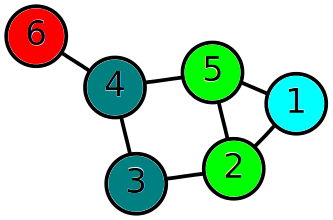
\includegraphics[width=\textwidth,height=0.25\textheight,keepaspectratio]{6n-graf.png}
    \end{itemize}
}

\frame{\frametitle{Cilk Model}
    \begin{itemize}
        \item Large shared memory
        \item Consistent caches between cores
        \item Synchronizing (or launching) $n$ tasks takes $T_\infty=\Th{\log n}$ time
        \item Cilk+ has this model with the addition of randomized work stealing \cite{cilk}
        \item BFS algorithms not using the Cilk Model
            \begin{itemize}
                \item Cray-BFS uses the Cray MTA-2 hardware model \cite{cray-bfs}
                \item Block-Queue-BFS uses the Intel Mic model \cite{block-queue-bfs}
            \end{itemize}

            \bigskip
            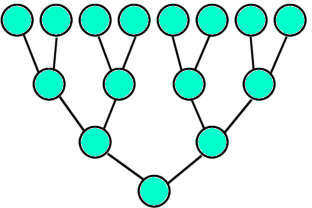
\includegraphics[width=\textwidth,height=0.25\textheight,keepaspectratio]{FullBinary.png}
    \end{itemize}
}

\frame{\frametitle{Level-Synchronous Parallel BFS in the Cilk Model}
    \begin{itemize}
        \item In the Cilk Model, Level-Synchronous BFS has a lower bound of $T_p = \Om{\frac{\size{\V}+\size{\E}}{p}+D\log p}$
        \item MIT-Bag-BFS uses penants, bags, and reducer hyperobjects \cite{mit-bag}
        \item Our new TBN-BFS algorithm
            \begin{itemize}
                \item Achieves the lower bound for $T_p, T_1, W_p$ in the worst case
                \item Is scale-free
                \item Can be implemented using Cilk+
                \item Can do its own scheduling deterministically
            \end{itemize}

            \bigskip
            \includegraphics[width=\textwidth,height=0.25\textheight,keepaspectratio]{jet-engine.jpg}
    \end{itemize}
}
%TODO ref MIT Cilk and/or Intel Cilk+

\frame{\frametitle{Serial-BFS}
    \begin{enumerate}
        \item for each vertex $u \in \V$
        \item \T $Dist_u \gets \infty$
        \item $Dist_s \gets 0$
        \item $Q \gets \emptyset$
        \item $\func{Enqueue}{Q, ~s}$
        \item while $Q \neq \emptyset$ do
        \item \T $u \gets \func{Dequeue}{Q}$
        \item \T for each vertex $v$ in $\Gamma(u)$ do
        \item \T \T if $Dist_v = \infty$ then
        \item \T \T \T $Dist_v \gets Dist_u + 1$
        \item \T \T \T $\func{Enqueue}{Q, v}$
    \end{enumerate}
}


\iffalse
optimal means:

$T_1 and T_P and W_P$ are asymptotically optimal. <- needs lower bound (parallel+level sync+cilk)
$T_P$ is something.
$T_1$ is something.
This is near perfect linear speedup when m is some function of blah and blah.

Next level:
The BSF algorithm runs on standard hardware and can be implemented using a multithreaded language such as Cilk or it can do its own scheduling.

Next level:
It's deterministically schedulable.

This algorithm is scale free, which means that Delta is the max degree of the graph and it doesn't require Delta to be bounded and Delta does not appear in any of the running times.


\fi

%TODO:
%TODO: What is parallel BFS?

%TODO: What is level synchronous BFS?
%      Quick comment about non-level synchronous BFS

%TODO: What is Cilk Model
%      Comment about algos in other models
%           PRAM, just timing, GPU, etc..
%
%       Lower bound in CILK model for level sync bfs


%       
%   Did BFS
%   Next?  Parallel or level synchronous?


\frame{\frametitle{Terminology}
    \begin{itemize}
        \item $n= \size{\V}$ the number of nodes in a graph \maybepause
        \item $m= \size{\E}$ the number of edges in a graph \maybepause
        \item $D= \Oh{n}$ the diameter of a graph \maybepause
        \item $\Gamma_u =$ the set of vertexes adjacent to $u$ \maybepause
        \item $T_s =$ the running time for a serial algorithm \maybepause
        \item $T_P =$ the running time for a parallel algorithm running on $P$ cores \maybepause
        \item $T_\infty =$ the running time for a parallel algorithm running on infinite cores
        \item $T_1 = \Om{T_s} =$ the running time for a parallel algorithm running on one core \maybepause
        \item $W_P = \Om{T_s} =$ the total work done by a parallel algorithm running on $P$ cores (excluding idle time)
            \begin{itemize}
                \item Reducing $W_P$ can reduce energy use \cite{race-to-idle}
            \end{itemize}
            %TODO: motivation for W_P
    \end{itemize}
}


\frame{\frametitle{Motivation for (P)BFS}
    BFS is used for
    \begin{itemize}
        \item Path Finding 
            \begin{itemize}
                \item Video Games
                \item Google Maps\maybepause
            \end{itemize}
        \item Analyzing social networks \maybepause %TODO: ref
        \item Designing and analyzing VLSI \maybepause %TODO: ref
        \item Task scheduling \maybepause %TODO: ref
        \item As a primitive in other algorithms
    \end{itemize}
}

\disableframe{\frametitle{Motivation for PBFS}
    BFS can achieve significant speedup for practical graphs
    %TODO: maybe delete this slide?  Or add more
}

\frame{\frametitle{Existing Algorithms}
    \begin{itemize}
        \item MIT-bag \cite{mit-bag} uses penants, bags, and reducer hyperobjects \pause
        \item block-queue-bfs \cite{block-queue-bfs} allocates space from FIFO in blocks \pause
        \item distinguished-bfs \cite{distinguished-bfs} contracts the graph to make it dense \pause
        \item cray-bfs \cite{cray-bfs} uses fast hardware mutexes and atomic increments
    \end{itemize}
}

\frame{\frametitle{General Approaches}
    \begin{itemize}
        \item Assumes PRAM model \maybepause
        \item Specialized for specific hardware \cite{blue-bfs}
            \begin{itemize}
                \item GPU
                \item CRAY (hardware mutex every $64$ bits, atomic add) \maybepause
                    \cite{cray-bfs}
            \end{itemize}
        \item Uses atomic instructions \cite{block-queue-bfs}
        \item Specialized for sparse (or dense) graphs only
        \item Specialized for bounded out-degree (not scale-free) \cite{mit-bag} \maybepause
        \item $T_1$ or $T_p$ is not asymptotically optimal \maybepause
        \item Room for energy efficiency improvements (non-optimal $W_P$) \maybepause
        \item Offloads some work to scheduler
            \begin{itemize}
                \item Work-stealing (randomized) gives high probability bounds
                    \cite{mit-bag}
            \end{itemize}
        \item Non level-synchronous \cite{distinguished-bfs}
    \end{itemize}
}

\disableframe{\frametitle{Bottlenecks for Parallelizing BFS}
    \begin{itemize}
        \item FIFO
        \item $Dist$ array
    \end{itemize}
}

\section{Clean BFS}
\frame{\frametitle{Clean BFS - Properties}
    \begin{itemize}
        \item Recall $T_s = \Oh{n+m}$
        \item $T_1 = \Oh{n+m}$ (optimal)
        \item $W_P = \Oh{n+m}$ (optimal)
        \item $T_P = \Oh{n/p+m/p+D\log P}$ (optimal)
        \item Scale-free
        \item Deterministic worst case bounds
    \end{itemize}
}

\frame{\frametitle{Clean BFS - High Level}
    For each level $\ell \in [0\ldots D)$
    \begin{enumerate}
        \item To get optimal $T_1,T_P$
        \begin{enumerate}
            \item Prepare to Split Work
            \item Split Work and Process Edges
            \item Dedup Vertexes and Combine Queues
        \end{enumerate}
    \item To get optimal $W_P$
        \begin{enumerate}
            \item Reduce Search Space
            \item Dynamically Choose Number of Cores
        \end{enumerate}
    \end{enumerate}
}

\subsection{Algorithm}
\frame{\frametitle{Clean BFS - Prepare to Split Work}
    \begin{enumerate}
        \item One input queue $Q_{in}\subseteq \V$
            \begin{enumerate}
                \item Each vertex in $Q_{in}$ is unique
                \item $\forall u (u \in Q_{in} \Rightarrow Dist_u = \ell)$
                \item $\forall u (u \in Q_{in} \Rightarrow \size{\Gamma_u} > 0$
            \end{enumerate}
        \item Generate $OutDegrees[0\leq i<\size{Q_{in}}] = \size{\Gamma(Q_{in}[i])}$ in parallel
        \item Perform a parallel prefix sum on $OutDegrees$
            \begin{tabular}{r|l|l|l|l|l|l|}
                \cline{2-7}
                $Q_{in}=$ &1 & 3 & 2 & 4 & $\ldots$ & $\ldots$ \\ \cline{2-7}
  $OutDegrees_{before} =$ &1 & 3 & 2 & 4 & $\ldots$ & $\ldots$ \\ \cline{2-7}
  $OutDegrees_{after}  =$ &1 & 4 & 6 & 10 & $\ldots$ & $m_\ell$ \\ \cline{2-7}
            \end{tabular}
    \end{enumerate}
}

\frame{\frametitle{Clean BFS - Split Work and Process Edges}
    \begin{enumerate}
        \item Each core $i$ processes $m_\ell/P$ edges
            \begin{enumerate}
                \item searches $OutDegrees$ for $1+\floor{\frac{i ~ m_\ell}{P}}$ to find starting edge
                \item does $\Oh{\log \frac{n_\ell}{P} + \log P}$ work
                \item processes $\floor{\frac{m_\ell}{P}}$ consecutive edges
                    \begin{enumerate}
                        \item $Q_i \gets \emptyset$
                        \item for each edge $(u,v)$
                        \item \T if $Dist_v = \infty$ then
                        \item \T \T $Dist_v \gets Dist_u + 1$
                        \item \T \T $Owner_v \gets i$
                        \item \T \T $\func{Enqueue}{Q_i, v}$
                    \end{enumerate}
                \item Benign race conditions
            \end{enumerate}
    \end{enumerate}
}

\frame{\frametitle{Clean BFS - Dedup Vertexes and Combine Queues}
    \begin{enumerate}
        \item $Size_{-1} = 0$
        \item Each core $i$ uses $Owner$ to ensure each vertex lives in at most one output queue
            \begin{enumerate}
                \item $Q_i \gets \set{u \in Q_i : Owner_u = i}$
                \item $Size_i \gets \size{Q_i}$
            \end{enumerate}
        \item Perform a parallel prefix sum on $Size$
        \item Each core $i$ copies its queue back into $Q_{in}$ at offset $Size_{i-1}$
    \end{enumerate}
}

\frame{\frametitle{Clean BFS - Reduce Search Space}
    \begin{enumerate}
        \item $N \gets \size{OutDegrees}$
        \item Each core $i$
            \begin{enumerate}
                \item $FirstDegree \gets OutDegrees[\floor{\frac{iN}{P}}-1]$
                \item $FirstDegreeNext \gets OutDegrees[\floor{\frac{(i+1)N}{P}}-1]$
                \item $FirstCore \gets \ceil{\frac{P~ FirstDegree}{m_\ell}}$
                \item $LastCore \gets \ceil{\frac{P~ FirstDegreeNext}{m_\ell}}$
                \item parallel for $j \gets FirstCore$ to $LastCore$
                \item \T $SubList_j \gets i$
            \end{enumerate}
        \item Using $SubList_i$, core $i$ can search only $n_\ell/p$ indexes
        \item $W_P$ reduces from $\Oh{n+m+DP\log P}$ to $\Oh{n+m+DP}$
    \end{enumerate}
}

\frame{\frametitle{Clean BFS - Dynamically Choose Number of Cores}
    \begin{itemize}
        \item In ``Prepare to Split Work'', right after the parallel prefix sum, $P_\ell \gets \func{min}{m_\ell, P}$
        \item Use at most $P_\ell$ cores until next time $m_\ell$ is calculated
        \item This ensures the $\Oh{P_\ell}$ work every level is $\Oh{m_\ell}$
        \item $W_P$ reduces from $\Oh{n+m+DP}$ to $\Oh{n+m+D}=\Oh{n+m}$ (optimal)
    \end{itemize}
}

\frame{\frametitle{Conclusions}
    \begin{itemize}
        \item Clean BFS has optimal $T_1, T_P, W_P$ in our computation model
        \item TODO MORE?
    \end{itemize}
}

\frame{\frametitle{Future Work}
    \begin{itemize}
        \item Optimize Clean BFS for the PRAM model
            \begin{itemize}
                \item Clean BFS runs in same time for PRAM but is not asymptotically optimal
                \item Try using approximate parallel prefix sum \cite{Goldberg95optimaldeterministic}
            \end{itemize}
        \item Modify Clean BFS to remove false sharing
            \begin{itemize}
                \item Examine using an $\Oh{n}$ sort algorithm for levels where $m_\ell = \Omega{n^\frac{1}{c}}$
                \item Try to distribute work by cacheline
            \end{itemize}
        \item Examine non level-synchronous approaches
    \end{itemize}
}

\iffalse
        \item Combined over all levels
            \begin{itemize}
                \item $T_P = \Oh{n/P + m/P + D\log P}$
                \item $T_1 = \Oh{n+m}$
                \item $W_P = \Oh{n+m+DP\log P}$\maybepause
            \end{itemize}
        \item 
\fi



\begin{frame}[allowframebreaks]
    \frametitle{References}
    %\bibliographystyle{amsalpha}
    \bibliographystyle{apalike}
    \bibliography{../source/bib/paper.bib}
\end{frame}

\end{document}






%TODO:
Add figures/slides/references for:


False sharing
CILK+

Related work
    m




































\iffalse
%\subsection{Subsection no.1.1  }
%\frame{
%Without title somethink is missing.
%}


\section{Section no. 2}
\subsection{Lists I}
\frame{\frametitle{unnumbered lists}
\begin{itemize}
\item Introduction to  \LaTeX
\item Course 2
\item Termpapers and presentations with \LaTeX
\item Beamer class
\end{itemize}
}

\frame{\frametitle{lists with maybepause}
\begin{itemize}
\item Introduction to  \LaTeX \maybepause
\item Course 2 \maybepause
\item Termpapers and presentations with \LaTeX \maybepause
\item Beamer class
\end{itemize}
}

\subsection{Lists II}
\frame{\frametitle{numbered lists}
\begin{enumerate}
\item Introduction to  \LaTeX
\item Course 2
\item Termpapers and presentations with \LaTeX
\item Beamer class
\end{enumerate}
}
\frame{\frametitle{numbered lists with maybepause}
\begin{enumerate}
\item Introduction to  \LaTeX \maybepause
\item Course 2 \maybepause
\item Termpapers and presentations with \LaTeX \maybepause
\item Beamer class
\end{enumerate}
}

\section{Section no.3}
\subsection{Tables}
\frame{\frametitle{Tables}
\begin{tabular}{|c|c|c|}
\hline
\textbf{Date} & \textbf{Instructor} & \textbf{Title} \\
\hline
WS 04/05 & Sascha Frank & First steps with  \LaTeX  \\
\hline
SS 05 & Sascha Frank & \LaTeX \ Course serial \\
\hline
\end{tabular}}


\frame{\frametitle{Tables with maybepause}
\begin{tabular}{c c c}
A & B & C \\
\maybepause
1 & 2 & 3 \\
\maybepause
A & B & C \\
\end{tabular} }


\section{Section no. 4}
\subsection{blocs}
\frame{\frametitle{blocs}

\begin{block}{title of the bloc}
bloc text
\end{block}

\begin{exampleblock}{title of the bloc}
bloc text
\end{exampleblock}


\begin{alertblock}{title of the bloc}
bloc text
\end{alertblock}
}
\fi
